\section{比较基准、小容量渐近与参数量级}
\label{sec:scaling}
% D 批80位解析求值的展示舍入；不是新增优化结果。
\newcommand{\DfillE}{1.578386}
\newcommand{\DoptE}{1.529511}
\newcommand{\DdeltaE}{0.048874}
\newcommand{\DtimeFillE}{4.770479}
\newcommand{\DtimeOptE}{2.234177}
\newcommand{\DsbE}{0.547695}
\newcommand{\DreleaseE}{0.451664}
\newcommand{\DsavingE}{3.096477}
\newcommand{\DfillZ}{16.874737}
\newcommand{\DoptZ}{16.816902}
\newcommand{\DdeltaZ}{0.057835}
\newcommand{\DtimeFillZ}{32.524198}
\newcommand{\DtimeOptZ}{24.260293}
\newcommand{\DsbZ}{0.260205}
\newcommand{\DreleaseZ}{0.245414}
\newcommand{\DsavingZ}{0.342732}
\newcommand{\DsmallBetaError}{6.40}


\subsection{纯容量填充与比较指标}
取同一组常参数、物理初值和容量约束。设自然轨道有首次容量触点 $(s_1,K)$，
并且 $s_1\ge s_B$。本文的纯容量填充策略是：先取 $q=0$ 到该触点，
再以 $q=q_B(s)$ 维持 $i=K$ 直至 $s=h$，随后永久取 $q=0$。
最优策略与它共享等待段和从 $s_1$ 到 $s_B$ 的容量段，
随后从 $(s_B,K)$ 完全跟踪至安全端点 $(\bar s_B,\bar i_B)$，再永久取 $q=0$。
这一定义只用于上述共同容量入口的比较；自然容量触点不存在或 $s_1<s_B$ 的初值不套用以下尾段公式。
记 $J^*=V(x_0)$，并定义
\begin{equation}
 \Delta J:=J_{\rm fill}-J^*,\qquad
 T_+(q):=\int_0^\infty\one_{\{q(t)>0\}}\dd t.
 \label{eq:scaling-metrics}
\end{equation}
相对节省始终写作 $\Delta J/J_{\rm fill}$，以纯容量填充成本为分母。
正控制时长 $T_+$ 不包含初始的免费等待，也不同于带权强度成本 $J$。
由式\eqref{eq:boundary-cost}和\eqref{eq:q1-cost}，有精确关系
\begin{align}
 J_{\rm fill}&=C_B(s_1,h),&
 J^*&=C_B(s_1,s_B)+\frac1h\ln\frac K{\bar i_B},\notag\\
 \Delta J&=C_B(s_B,h)-\frac1h\ln\frac K{\bar i_B},&
 T_{+,\rm fill}&=T_B(s_1,h),\notag\\
 T_+^*&=T_B(s_1,s_B)+\frac1\gamma\ln\frac K{\bar i_B}.&&
 \label{eq:common-capacity-comparison}
\end{align}
因而成本差与正控制时长差均由公共尾段决定，退出容量的位置分别为 $h$ 和 $s_B$。
两策略具有同一初始等待时间，所以其永久解除时刻之差也等于正控制时长之差；
最优策略在 $\bar s_B>h$ 处进入安全集，纯容量填充则在 $(h,K)$ 解除。

例如，原有 E2 的参数为 $\beta=0.5,c=2,\gamma=0.3,K=0.15$，初值为 $(0.99,0.01)$。
解析公式给出 $J_{\rm fill}=\DfillE$、$J^*=\DoptE$、$\Delta J=\DdeltaE$，
相对节省为 $\DsavingE\%$，与前节的 $3.10\%$ 是同一比较。
相应的 $T_{+,\rm fill}=\DtimeFillE$、$T_+^*=\DtimeOptE$，容量退出位置为
$h=0.3$ 与 $s_B=\DsbE$，最优解除位置为 $\bar s_B=\DreleaseE$。
这里的时间单位与参数速率的单位对应；该算例是数学示例。

\subsection{固定传播概率下的小容量命题}
\begin{proposition}[小容量的成本与时长标度]
\label{prop:small-capacity}
固定 $0<\beta<1$、$c,\gamma>0$，并假设 $h=\gamma/(\beta c)<1$。
考虑物理可行初值族 $(s_0(K),i_0(K))$，其中 $0<i_0(K)\le K$，
自然容量触点存在，且 $s_1(K)\to s_1^\circ>h$。
当 $K\downarrow0$ 时，两策略最终具有共同容量入口，且
\begin{align}
 s_B-h&=\frac K\beta-\frac{(1-\beta)K^2}{\beta^3h}+O(K^3),
 \label{eq:small-K-switch}\\
 \Delta J&=\frac{K^2}{24\beta^4h^3}+O(K^3),
 \label{eq:small-K-cost}\\
 T_{+,\rm fill}-T_+^*&=\frac1{\beta\gamma}+O(K).
 \label{eq:small-K-time}
\end{align}
令
\begin{equation}
 \mathcal C(S):=\frac\beta{1-\beta}
 \left[\ln\frac Sh-\beta\ln\frac{S-p}{\ell}\right],\qquad S>h.
 \label{eq:small-K-C}
\end{equation}
则 $\mathcal C(S)>0$，并且
\begin{equation}
 J_{\rm fill}\sim\frac{\mathcal C(s_1^\circ)}K,\qquad
 \frac{\Delta J}{J_{\rm fill}}
 \sim\frac{K^3}{24\beta^4h^3\mathcal C(s_1^\circ)}.
 \label{eq:small-K-relative}
\end{equation}
式\eqref{eq:small-K-switch}--\eqref{eq:small-K-time}的余项对固定参数及上述共同入口统一，
不声称对 $\beta\downarrow0$ 一致。
\end{proposition}
完整证明见附录\ref{app:small-capacity-proof}。
绝对节省为 $K^2$ 阶，而纯填充成本为 $K^{-1}$ 阶，故相对节省为 $K^3$ 阶。
时长差趋于正常数的同时，两者时长均为 $K^{-1}$ 阶，因而 $T_+^*/T_{+,\rm fill}\to1$。
这不意味着成本最优策略同时最小化正控制时长。

首项用于说明标度，在小 $\beta$ 下不能直接当作有限 $K$ 的准确估计。
附录的进一步展开给出 $\Delta J$ 首项的相对修正尺度为 $K/(\beta^2h)$。
以 $\beta=0.155$ 为例，表\ref{tab:parameter-sources}中文献示例的
$c=10,\gamma=0.3504$ 下，$K=10^{-4}$ 时解析成本差与渐近首项的偏差，
以该首项为分母仍约为 $\DsmallBetaError\%$；精度随参数与误差指标改变。
因此，图\ref{fig:scaling}采用解析公式的高精度求值。

\subsection{参数来源与解析扫描}
表\ref{tab:parameter-sources}区分本文示例、文献估计和本文作者新拟合。
本文 E1--E5 保持原有数学示例的含义。
\citet[第8节，表1]{Zhou2024SPCI}的西安拟合对应
$\gamma=\delta_I+\gamma_I=0.1998+0.1006=0.3004$；
其常规阶段仍有 $q_0=0.4624$，而本文无控制基准为绝对跟踪比例 $q=0$。
因而不能将文献的常规阶段再生数与本文无控制再生数直接混用。
\citet[表1]{He2023TDINN}的六地传播概率估计范围为 $0.1281$--$0.2544$；
其接触率和跟踪比例为数据推断的时变函数，不把这些概率与另一文献的接触率拼成已校准参数组。
\begin{table}[htbp]
\centering\small
\caption{用于解释量级的参数来源。$\beta$ 无量纲；Zhou 等的时间单位为日，
本文引用其速率时沿用日。文献参数的引用不等于对本稿控制问题重新拟合。}
\label{tab:parameter-sources}
\begin{tabularx}{\linewidth}{@{}>{\raggedright\arraybackslash}p{2.8cm}>{\raggedright\arraybackslash}p{3.7cm}>{\raggedright\arraybackslash}X@{}}
\toprule
类别与场景 & 参数 & 来源与使用范围\\
\midrule
本文数学示例 & $\beta=0.5$, $c=2$, $\gamma=0.3$ & E1--E5 的结构基准；$K=0.15$，不指定现实人口。\\
文献模拟示例 & $\beta=0.155$, $c=10$, $\gamma=0.3504$ & Zhou 等图6、图12；用于小概率下的渐近精度核对，不称西安拟合。\\
文献西安拟合 & $\beta=0.13675$, $c_0=10.1317$, $\gamma=0.3004$ & Zhou 等表1；仅抽取常规接触率构造常参数无回流情景；$q_0=0.4624$ 不用作本文的零控制。\\
文献六地估计 & $\beta\in[0.1281,0.2544]$ & He--Tang--Xiao 表1；仅说明概率量级，不合并各地或跨文献的拟合参数。\\
本文作者新拟合 & 无 & 本文不据此表声称新的数据拟合或城市政策复现。\\
\bottomrule
\end{tabularx}
\end{table}

两篇文献的原模型均使用人数仓室，本文统一按 $s=S/N,i=I/N$ 归一化。
Zhou 等的西安表列出 $S_0=12952907,I_0=2,H_0=1$，未单列独立的 $N$；
本文的比例初值另行设定，不从该表反推实际初始负荷。
其 $\delta_q=0.2001$ 不进入闭合的 $(s,i)$ 子系统，故不参与以下成本计算。
He 等基于日度观测估计时变速率，本文仅引用其无量纲 $\beta$，不转用各地人口或速率。

图\ref{fig:scaling}固定 $\beta c=1$、$\gamma=0.3$，所以 $h=0.3$ 不变，
改变 $\beta$ 时同步取 $c=1/\beta$、$\ell=\beta h$、$p=(1-\beta)h$。
扫描取 $\beta\in\{0.13,0.155,0.25,0.5,0.8\}$、$10^{-4}\le K\le0.15$，
固定初值 $(s_0,i_0)=(0.9999,0.0001)$，仅在 $s_1\ge s_B$ 的共同容量分支上报告比较。
共620组参数中，$\beta=0.13,K=0.15$ 的一组满足 $s_1<s_B$，故不计入共同尾段的成本与时长曲线。
这用于分离跟踪机制对量级的影响，不表示同一疾病的传播概率与接触率可任意独立调整。
此外，用 $s_0(K)=1-K/2,i_0(K)=K/2$ 的初值族单独核对 $K\downarrow0$ 的归一化比值，
不把固定正 $i_0$ 的扫描向 $K<i_0$ 延拓。
所有值由80位精度的标量方程和闭式弧成本求得；微小收益直接计算公共尾段差，
不以双精度总成本相减识别 $K^2$ 项。
\begin{figure}[htbp]
\centering
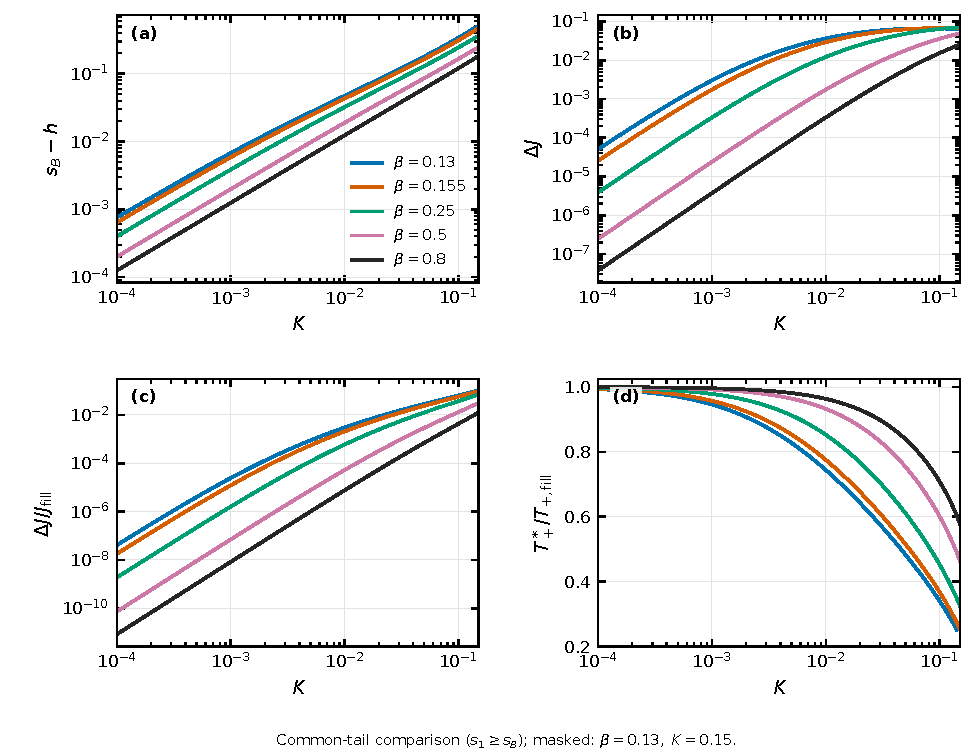
\includegraphics[width=\linewidth]{../validation/scaling_asymptotics_20261021/magnitude.pdf}
\caption{固定 $\beta c$ 与 $\gamma$ 的无回流解析量级扫描。
四幅图分别给出提前退出容量的距离、绝对成本节省、以纯填充成本为分母的相对节省，
以及正控制时长比。比较使用相同参数、初值和容量；曲线仅表示所述解析模型，未新增配点求解。}
\label{fig:scaling}
\end{figure}

作为来源明确的另一情景，取 Zhou 等西安拟合的 $\beta,c_0,\gamma$，
并另设容量 $K=0.01$，初值仍为 $(0.9999,0.0001)$。
所得 $J_{\rm fill}=\DfillZ$、$J^*=\DoptZ$、$\Delta J=\DdeltaZ$，
相对节省为 $\DsavingZ\%$，正控制时长为 $\DtimeFillZ$ 日与 $\DtimeOptZ$ 日。
该容量和初值属于本文的情景设定，不能解释为西安实际容量、实际初始感染比例或原文时变拟合的复现。
